% *********************************************************************
% © 2021-2022 Jeremy Sylvestre
%
% Permission is granted to copy, distribute and/or modify this document
% under the terms of the GNU Free Documentation License, Version 1.3 or
% any later version published by the Free Software Foundation; with no
% Invariant Sections, no Front-Cover Texts, and no Back-Cover Texts. A
% copy of the license is included in the appendix entitled “GNU Free
% Documentation License” that appears in the output document of this
% PreTeXt source code. All trademarks™ are the registered® marks of
% their respective owners.
%
% *********************************************************************

\newcommand*{\xmin}{-0.5}
\newcommand*{\xmax}{6.5}
\newcommand*{\ymin}{-5}
\newcommand*{\ymax}{50}

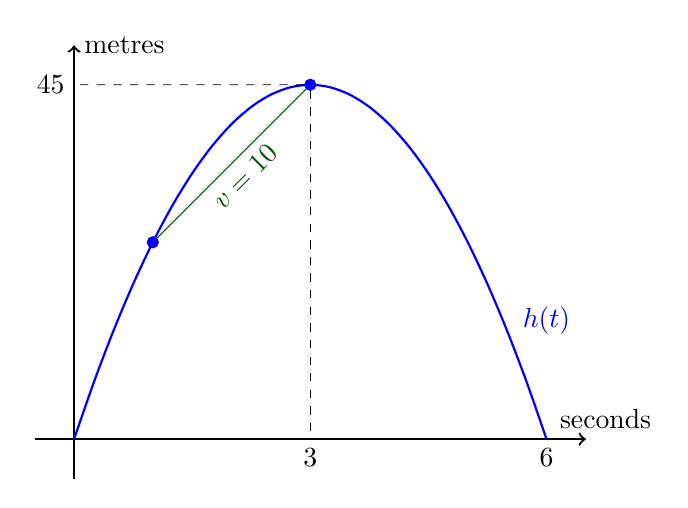
\begin{tikzpicture}
[
	closedpt/.style={circle,draw,fill,inner sep=0pt,minimum size=4pt},
	openpt/.style={circle,draw,inner sep=0pt,minimum size=4pt},
	yscale=0.1
]

	% v0 = 30, g = 10

	% axes
	\draw[->,thick] (\xmin,0) -- (\xmax,0) node[above,xshift=0.25cm] {seconds};
	\draw[->,thick] (0,\ymin) -- (0,\ymax) node[right] {metres};

	% position
	\draw[blue,thick,domain=0:6,smooth] plot (\x,{- 5 * \x * \x + 30 * \x});
	\node[blue] at (6,15) {$h(t)$};

	\node[below] at (6,0) {$6$};

	\node[closedpt,blue] at (1,25) (start) {};
	\node[closedpt,blue] at (3,45) (max) {};

	\draw[dashed, very thin] (max) -- (3,0) node[below] {$3$};
	\draw[dashed, very thin] (max) -- (0,45) node[left] {$45$};

	\draw[green!33!black] (start) to node[below,rotate=45] {$\avg{v} = 10$} (max);

\end{tikzpicture}
